\hypertarget{Design}{\chapter{Design}}

\section{Motivace}

Při tvorbě aplikace bylo neustále nutné myslet na dva hlavní faktory, kolem kterých se celý design musí odvíjet; program je určený pro dvě skupiny: učitele a~žáky zároveň. 

Úkolem žáka je v časovém limitu odpovědět na jazykové otázky. Žák by měl mít co nejméně možností jak podvádět, aby byl správně umístěn do jazykové skupiny úměrné jeho znalostem; dostane náhodnou sadu otázek různých obtížností, které pro jeho ročník navolí učitel.

Učitel pracuje se svým vlastním rozhraním, kde zadává otázky, vytváří testy, \mbox{kontroluje} průběh testování a získává automaticky zpracované výsledky.

V obou případech je důležité, aby byla webová aplikace intuitivní na používání, měla příjemný design a hlavně spolehlivě fungovala.

\section{Přihlašování}
\label{sec:login-design}

Ještě před tím, než se uživatelé dostanou do svého rozhraní, je potřeba, aby se přihlásili. Tato část aplikace je společná pro žáky i učitele. 

\begin{figure}[H]
    \centering
    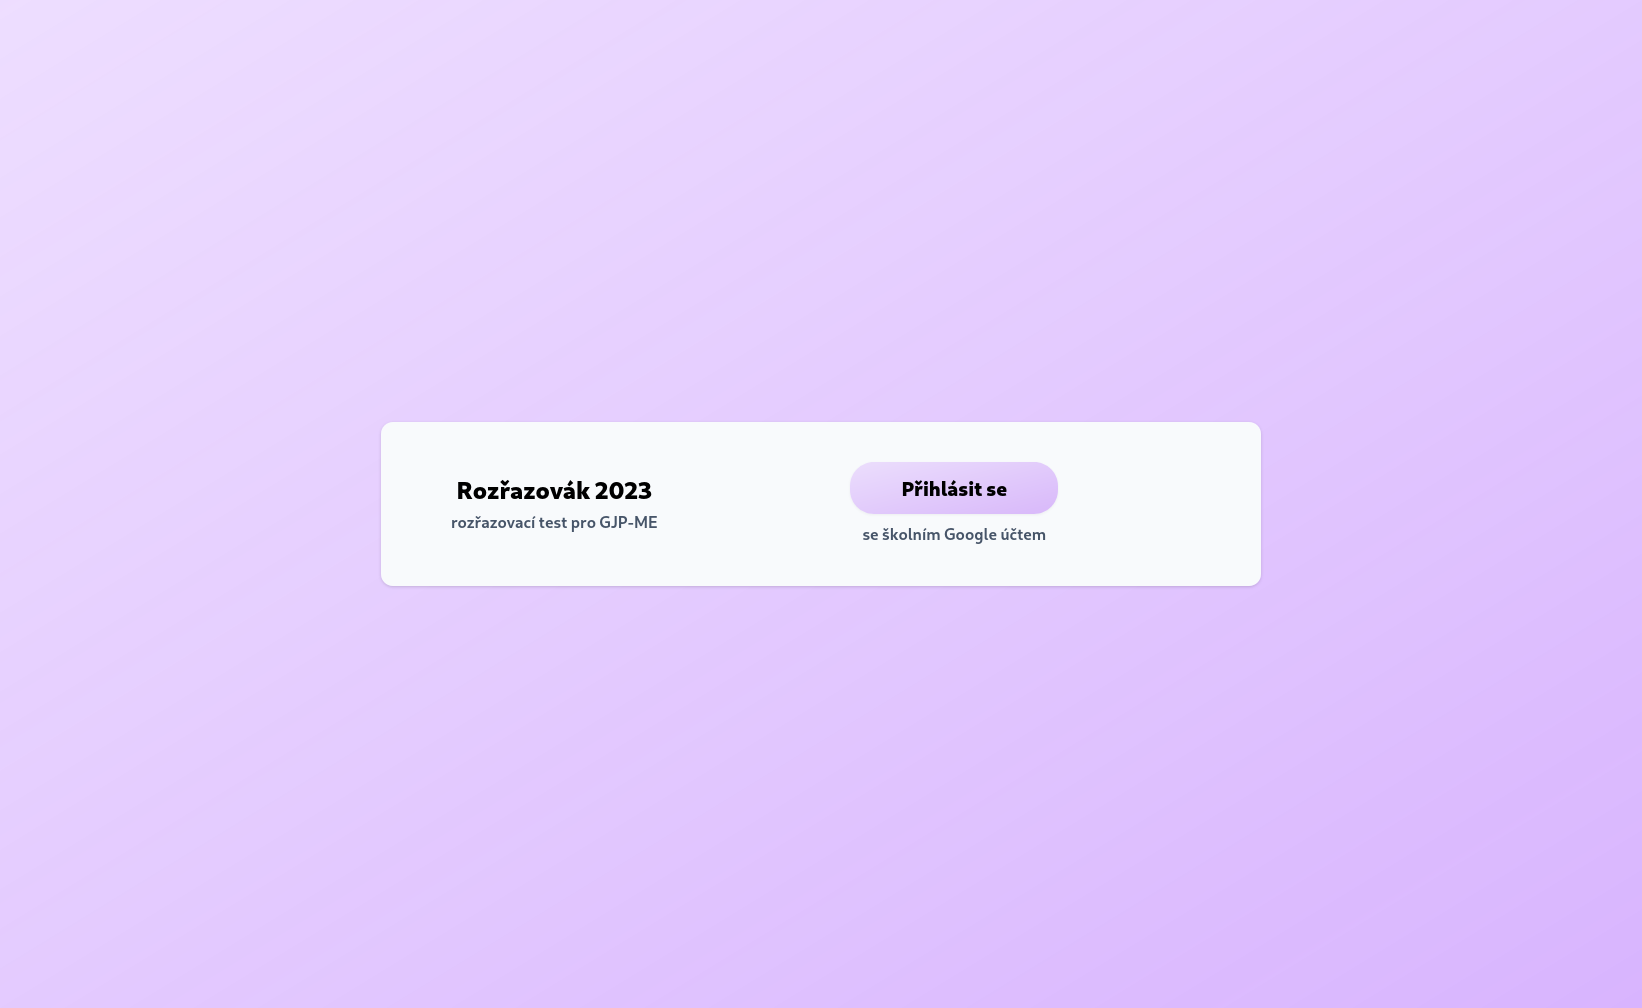
\includegraphics[width=350px]{images/01design/login.png}
    \caption{Přihlašovací stránka je hlavní stránkou aplikace.}
\end{figure}

Učitelé a žáci se přihlásí pomocí svého školního Google účtu (viz \ref{sec:login}).

\newpage

Pokud se přihlásí učitel, zobrazí se nabídka pro přechod do administrátorské sekce.

\begin{figure}[H]
    \centering
    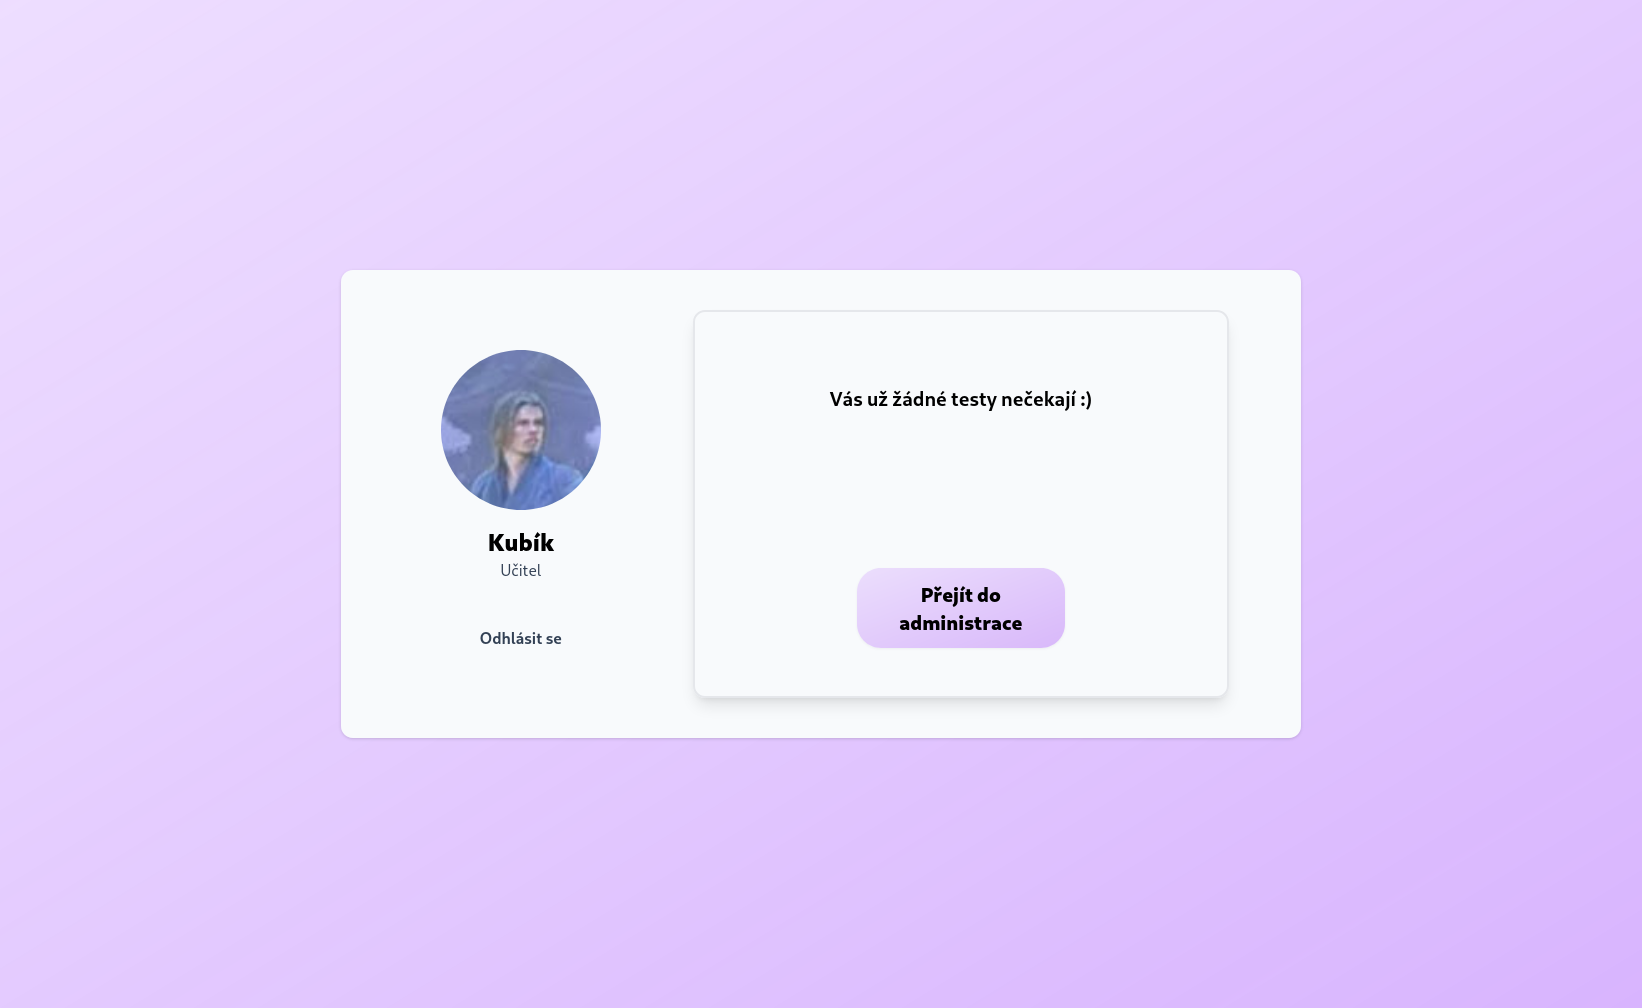
\includegraphics[width=350px]{images/01design/teacher.png}
    \caption{Hlavní stránka po přihlášení učitele.}
\end{figure}

Pokud se přihlásí žák, ve výchozím stavu se mu zobrazí stránka s informací, že pro něj aktuálně není spuštěný žádný test.

\begin{figure}[H]
    \centering
    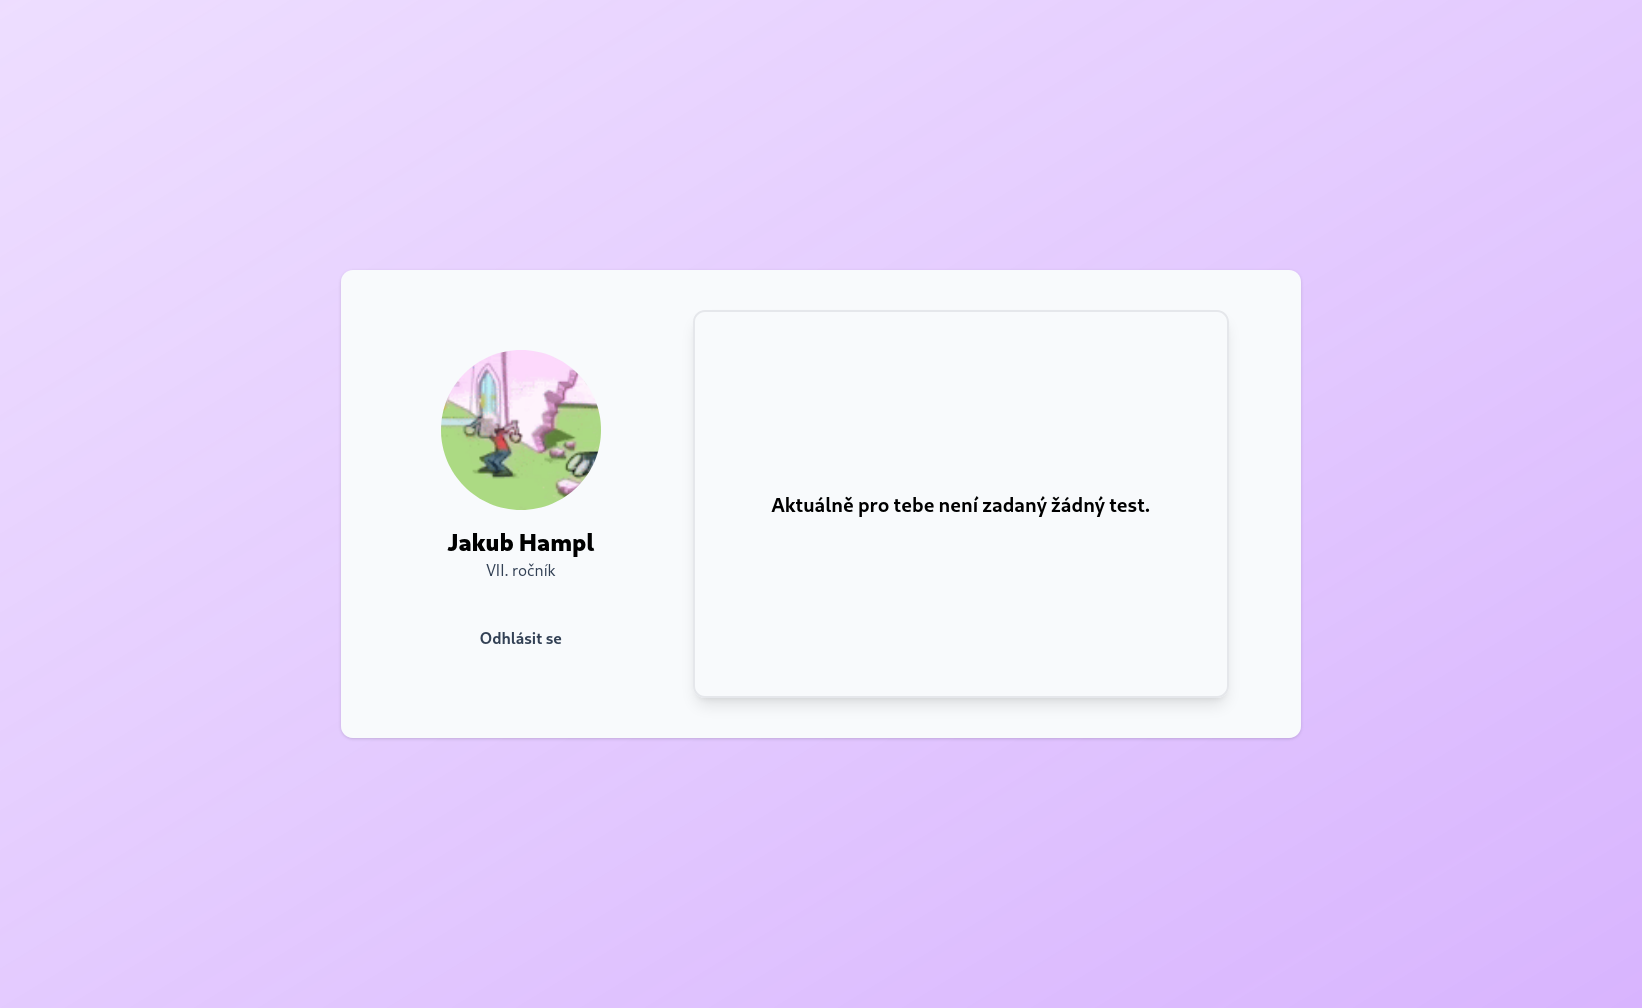
\includegraphics[width=350px]{images/01design/student-no-test.png}
    \caption{Hlavní stránka po přihlášení žáka bez zadaného testu.}
\end{figure}

Pokud je pro ročník přihlášeného žáka aktuálně aktivovaný test, je vidět jeho časové omezení, počet otázek a obtížnost. Pokud ne, zobrazí se pouze informace o tom, že pro žáka žádný test aktuálně spuštěný není.

\begin{figure}[H]
    \centering
    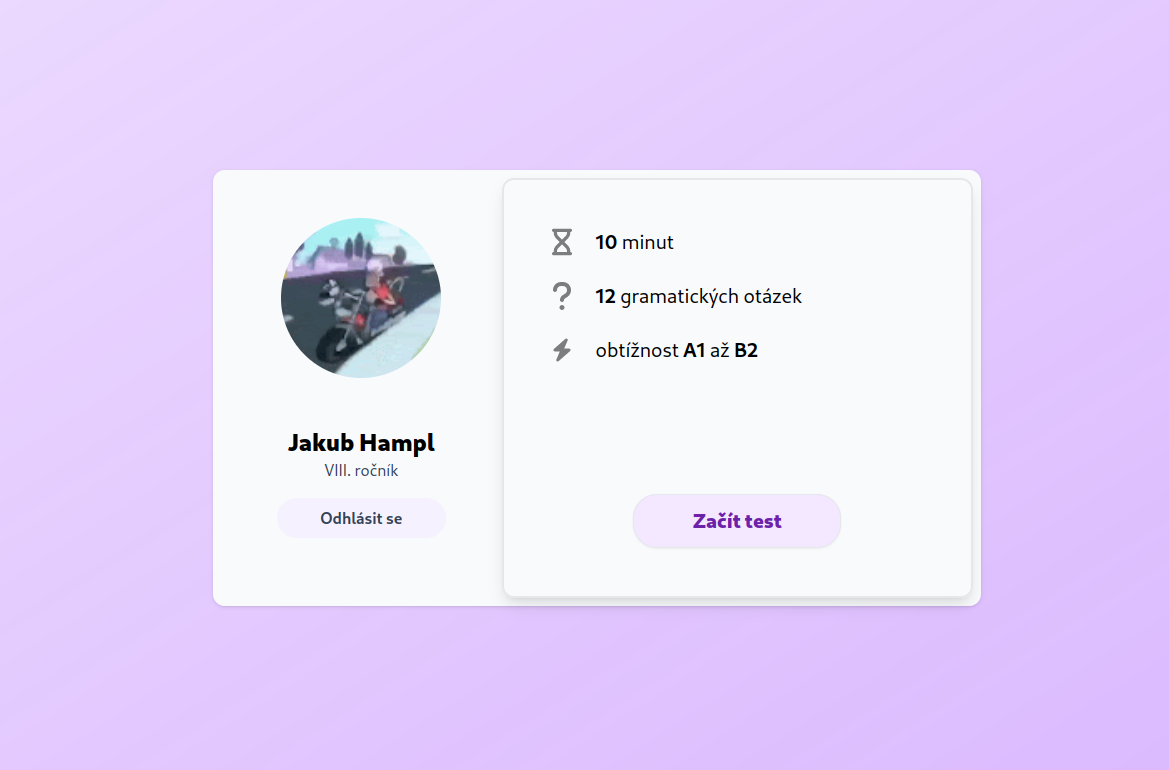
\includegraphics[width=350px]{images/01design/student-yes-test.png}
    \caption{Hlavní stránka po přihlášení žáka se zadaným testem.}
\end{figure}

Při aktivovaném testu může žák test spustit. Po spuštění se pro žáka vygeneruje originální sada otázek (viz \ref{userapi}) a žák je přesměrován do žákovského rozhraní. Pokud žák během testu tuto stránku opustí (například kvůli technickým potížím, výpadku proudu, atp.), zůstává test spuštěný a je možné pokračovat v jeho vyplňování z hlavní stránky. 

\begin{figure}[H]
    \centering
    
\includegraphics[width=200px]{images/01design/continue.png}
    \caption{Při probíhajícím testu se text tlačítka změní na "Pokračovat" a zobrazí se pod ním zbývající čas.}
\end{figure}

Jakmile žák test odevzdá, je přesměrován zpět na hlavní stránku, kde mu je sdělen jeho výsledek.

\begin{figure}[H]
    \centering
    
\includegraphics[width=350px]{images/01design/filled-out.png}
    \caption{Hlavní stránka s výsledky po odevzdání testu.}
\end{figure}

V případě, že žák na testování chyběl a stránku si zobrazí poté, co je test učitelem ukončen, zobrazí se mu tato informační stránka.

\begin{figure}[H]
    \centering
    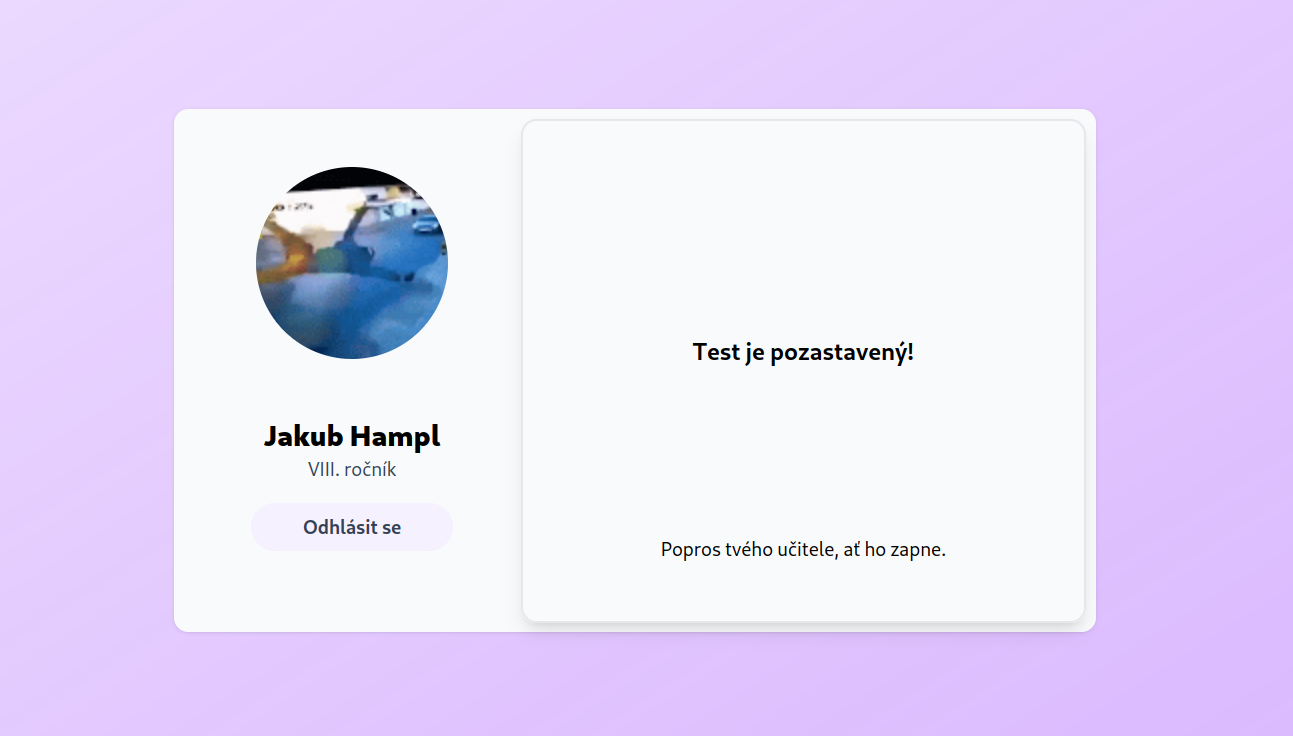
\includegraphics[width=350px]{images/01design/pending.png}
    \caption{Hlavní stránka s informací o pozastavení testu.}
\end{figure}

\section{Žákovské rozhraní}

Žákovské rozhraní slouží k vyplňování vygenerovaných testů. Pro každý ročník je předem nastavený čas a počet otázek různých obtížností (viz \ref{adminapi}). Z banky otázek je podle těchto kritérií několik náhodně vybráno a zobrazeno. Otázky mohou být různého druhu, ale u každé otázky je vždy na výběr ze čtyř možností, z nichž právě jedna je správná. V pravém horním rohu každé otázky lze slabě vidět ID otázky (pro usnadnění komunikace s učitelem, například pokud student v otázce najde chybu).

\begin{figure}[H]
    \centering
    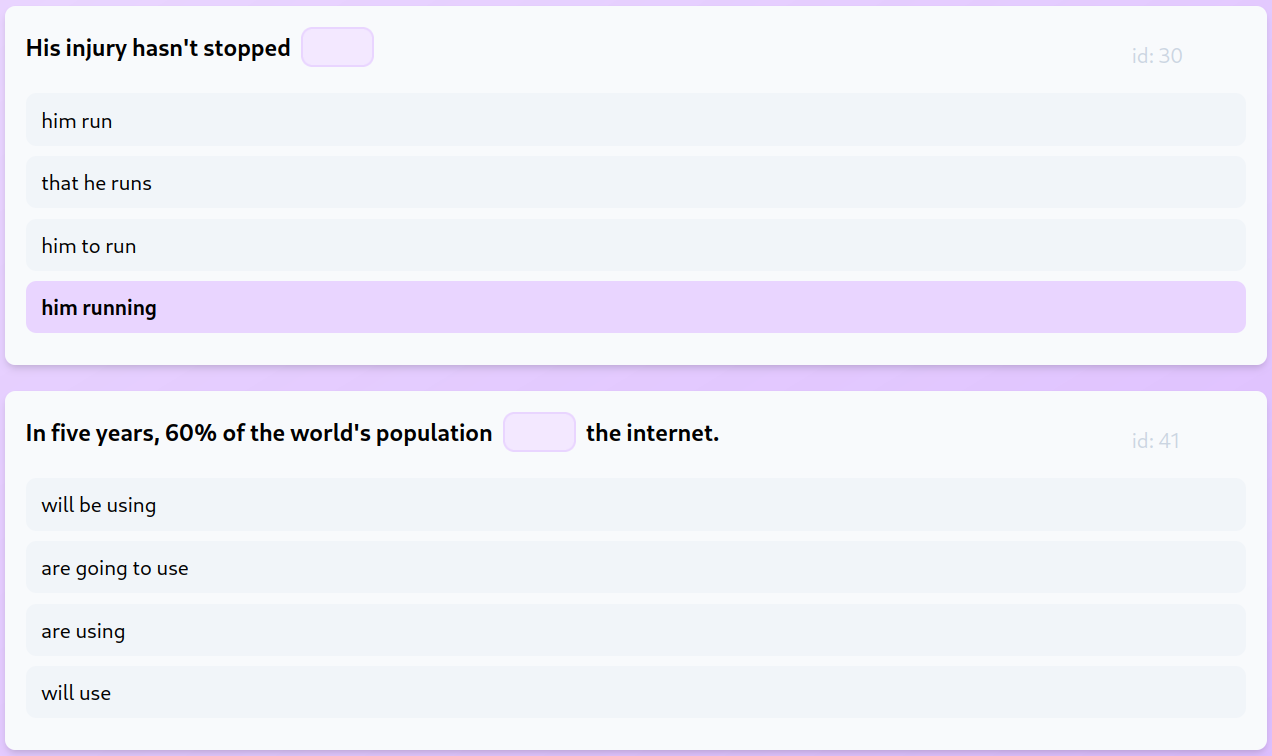
\includegraphics[width=400px]{images/01design/otazky.png}
    \caption{Dvě vygenerované otázky. Tmavě fialové zbarvení značí výběr.}
    \label{purplerect}
\end{figure}

\begin{figure}[H]
    \centering
    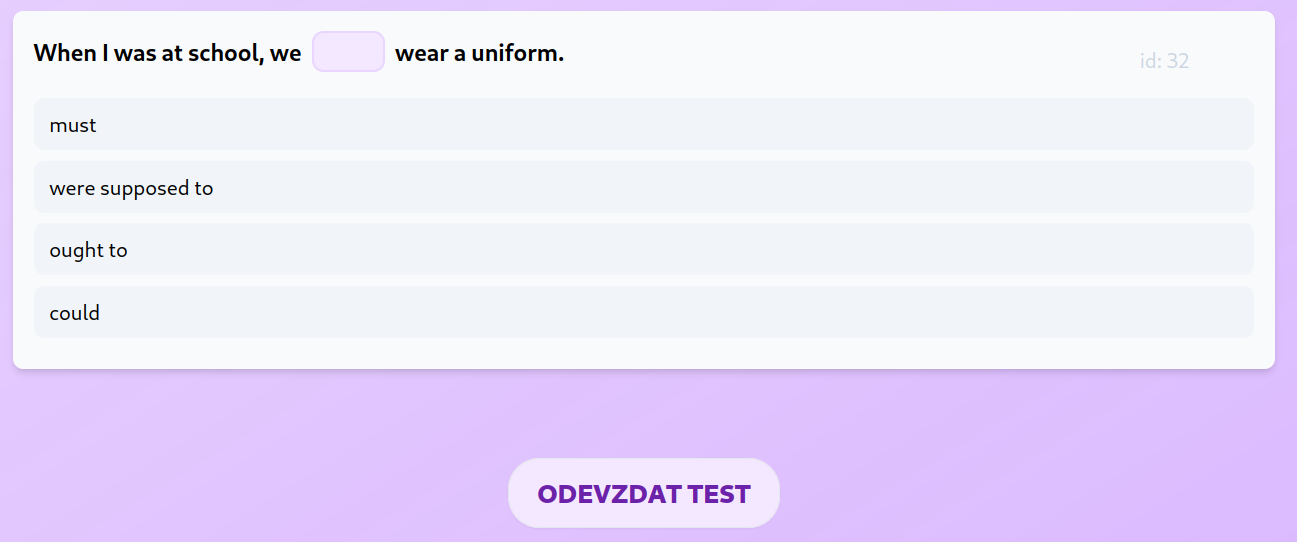
\includegraphics[width=400px]{images/01design/submit.png}
    \caption{Otázka a tlačítko pro odevzdání testu.}
\end{figure}

Po vyplnění testu může žák test odevzdat stisknutím tlačítka. Pokud tak neučiní do konce časového limitu, test se odevzdá sám. Po odevzdání testu je uživatel přesměrován zpět na hlavní stránku.

\section{Učitelské rozhraní}
\label{sec:admin}

Učitelské rozhraní je poměrně komplikované, proto je rozděleno do několika částí. V těchto částech se lze pohybovat pomocí takzvaného \enquote{navbaru}, který se nachází v~horní části obrazovky.

\begin{figure}[H]
    \centering
    
\includegraphics[width=400px]{images/01design/navbar.png}
    \caption{Navbar v učitelském rozhraní.}
\end{figure}

Na jeho levé straně můžeme přepínat do různých částí programu; aktuálně vybranou část značí fialový obrys. Na pravé straně lze vidět uživatelské jméno a možnost odhlásit se.

Po přechodu do administrátorské sekce se učitel dostane do záložky \enquote{Přehled}, kde je prozatím vidět pouze aktuální počet spuštěných testů.

\subsection{Testy}

Tato sekce programu slouží ke správě testů a ke stahování zpracovaných výsledků.

\begin{figure}[H]
    \centering
    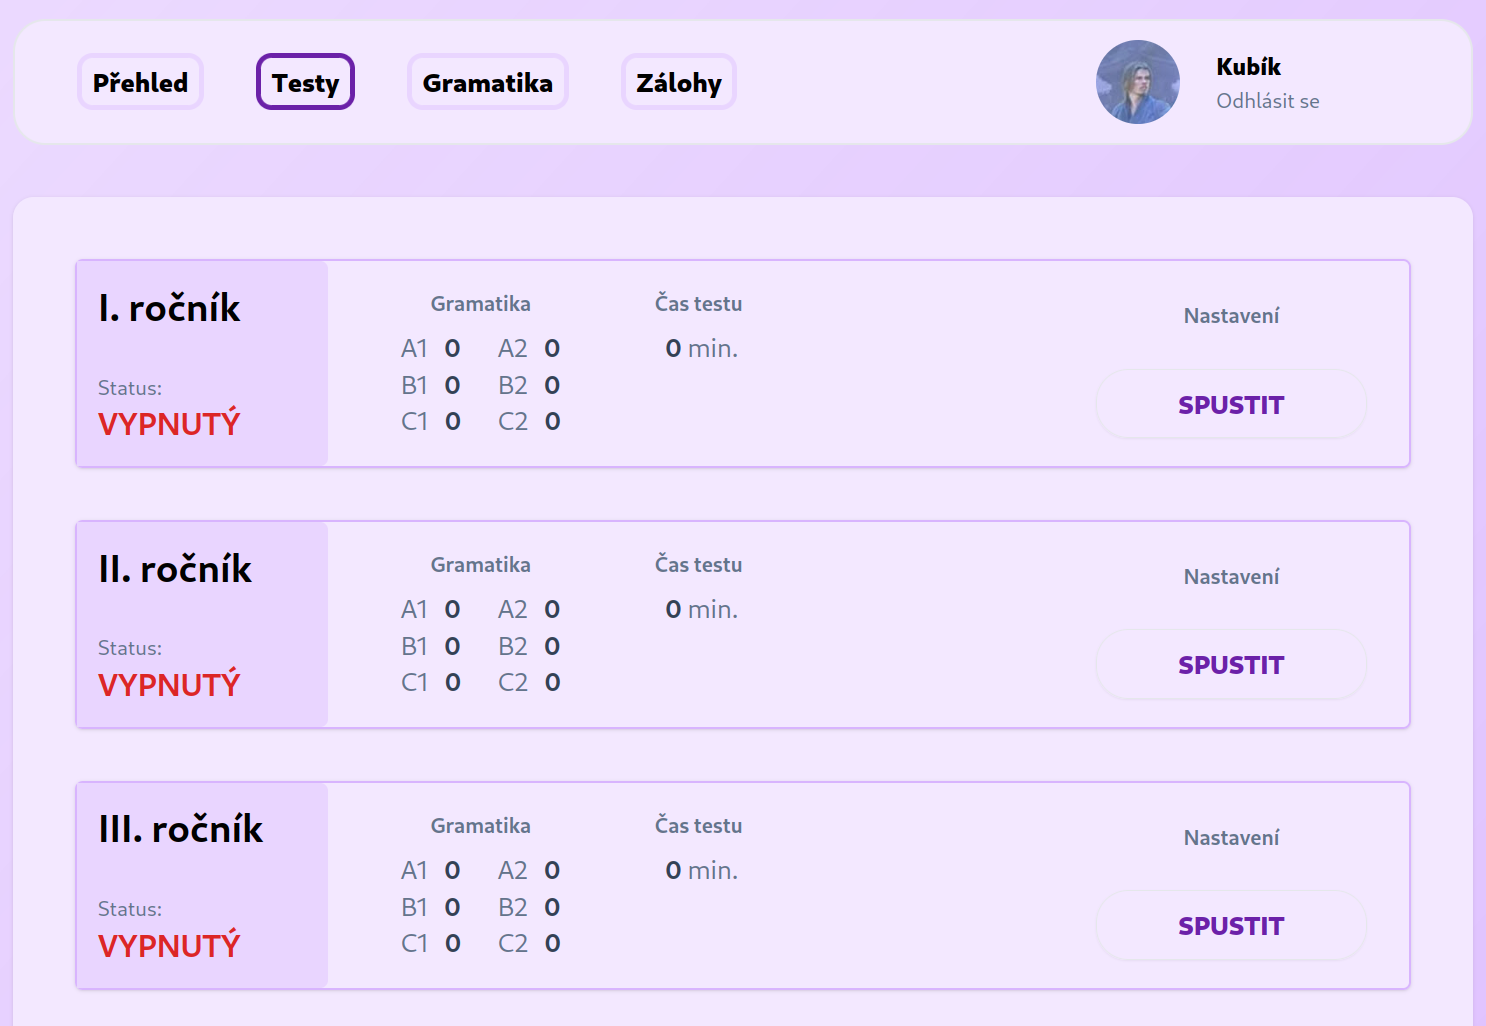
\includegraphics[width=400px]{images/01design/tests.png}
    \caption{Sekce Testy.}
\end{figure}

Při prvotním spuštění programu se automaticky vygeneruje osm testů (pro osm ročníků) s identickým výchozím nastavením. 

\begin{figure}[H]
    \centering
    
\includegraphics[width=400px]{images/01design/test.png}
    \caption{Detail komponentu testu.}
\end{figure}

V levé části se nachází číslo ročníku a status testu (\M{VYPNUTÝ}, \M{AKTIVNÍ} a~\M{VYPLNĚNÝ}). Ve sloupci Gramatika lze vidět počet použitých otázek pro každou jazykovou obtížnost. Ve sloupci Čas testu lze vidět časový limit v minutách. Úplně vpravo pak tlačítka pro nastavení a spuštění testu.

\begin{figure}[H]
    \centering
    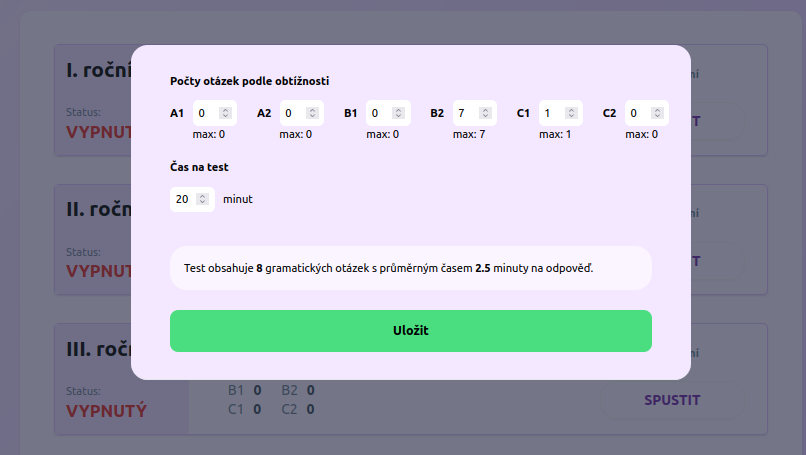
\includegraphics[width=400px]{images/01design/test-modal.png}
    \caption{Modální okno nastavení testu.}
\end{figure}

V modálním\footnote{Modální okno je typ uživatelského rozhraní, které vynucuje interakci s uživatelem, dokud není dokončena nebo zrušena. Tato okna se často zobrazují před ostatním obsahem na obrazovce.} okně nastavení lze změnit hodnoty pro použití otázek pro každou jazykovou obtížnost, níže i čas na test. Všechny zadané informace jsou shrnuty ve větě, která se během zadávání dat živě aktualizuje.

Tlačítko \M{Uložit} je zde spíše pro efekt, protože se stejně vše po zavření okna automaticky uloží.

Po zmáčknutí tlačítka \M{Spustit} se test spustí, což je reflektováno ve statusu testu a~v~zablokování možnosti Nastavení. V tomto stavu máme pouze možnost test zastavit.

\begin{figure}[H]
    \centering
    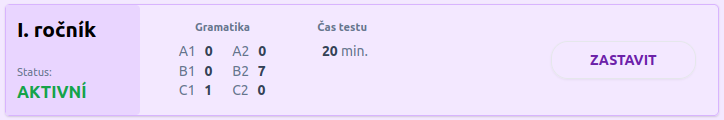
\includegraphics[width=400px]{images/01design/test-running.png}
    \caption{Detail spuštěného testu.}
\end{figure}

Po zastavení testu se status změní na \M{VYPLNĚNÝ}. Z tohoto stavu lze test znovu spustit tlačítkem \M{Restartovat} (toto je například potřeba, pokud během rozřazovacích testů někdo chyběl, což je poměrně pravděpodobné), \M{Smazat výsl}{edky} (tato možnost test dostane zpět do stavu \M{VYPNUTÝ} a je nevratná) a nebo si stáhnout výsledky ve formátu \M{.xlsx} (Excel tabulka).

\begin{figure}[H]
    \centering
    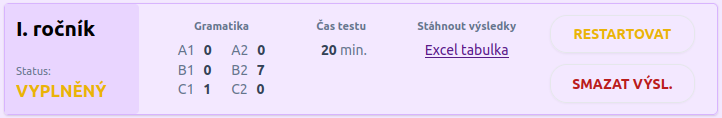
\includegraphics[width=400px]{images/01design/test-filled.png}
    \caption{Detail vyplněného testu.}
\end{figure}

Výsledná tabulka má sloupce pro jméno, e-mail, procentuální úspěšnost, získané body a ID špatně zodpovězených otázek (viz program \ref{xslxgen}). Řádky jsou seřazeny sestupně dle úspěšnosti.

\subsection{Gramatika}

Sekce Gramatika slouží k upravování gramatických otázek. Skládá se ze seznamu uložených otázek v databázi. V rychlém náhledu můžeme vidět text otázky, správnou odpověď, jazykovou úroveň a ID. V horním pravém rohu této sekce se nachází tlačítko pro vytvoření nové otázky. Stejné tlačítko se nachází i na konci seznamu.

\begin{figure}[H]
    \centering
    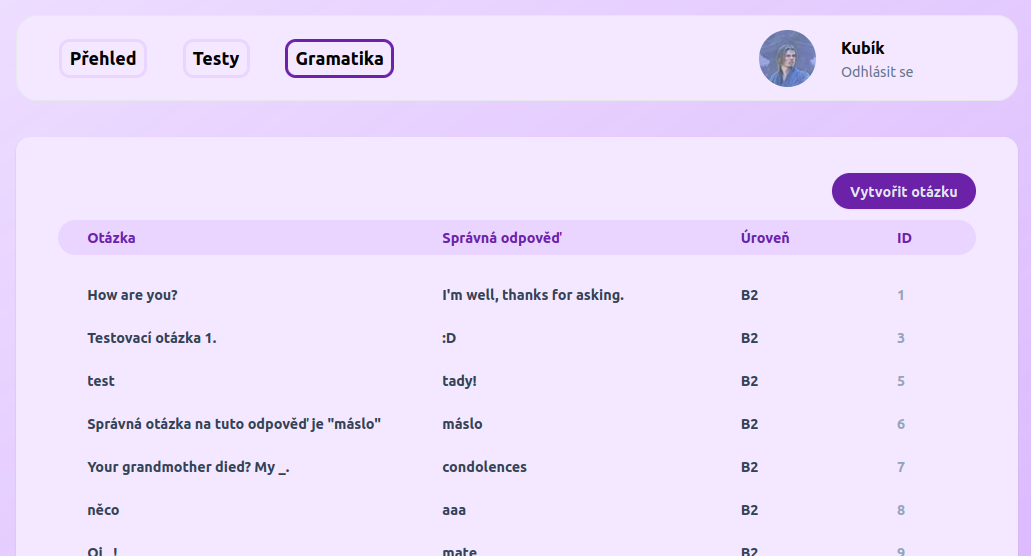
\includegraphics[width=400px]{images/01design/grammar.png}
    \caption{Sekce Gramatika.}
\end{figure}

Po kliknutí na otázku se otevře modální okno s nastavením dané otázky. Při kliknutí na tlačítko pro vytvoření otázky se otevře stejné okno, akorát nevyplněné. Zde je potřeba vyplnit text otázky, správnou odpověď, tři špatné odpovědi a vybrat jednu z jazykových obtížností. 

\begin{figure}[H]
    \centering
    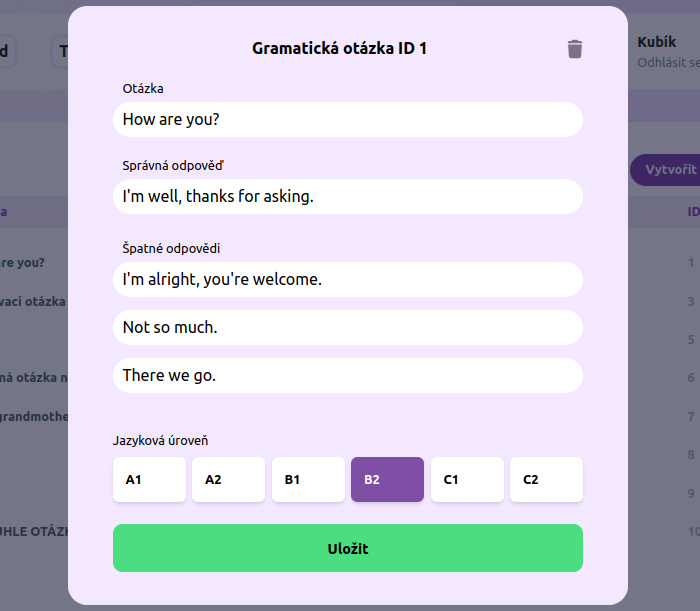
\includegraphics[width=400px]{images/01design/question.png}
    \caption{Modální okno nastavení gramatické otázky.}
    \label{questionfill}
\end{figure}

Program automaticky kontroluje správnost zadaných údajů -- zdali se nějaká ze špatných odpovědí neshoduje se správnou a zdali jsou všechna políčka vyplněná. Výchozí hodnota jazykové obtížnosti je A1.

\begin{figure}[H]
    \centering
    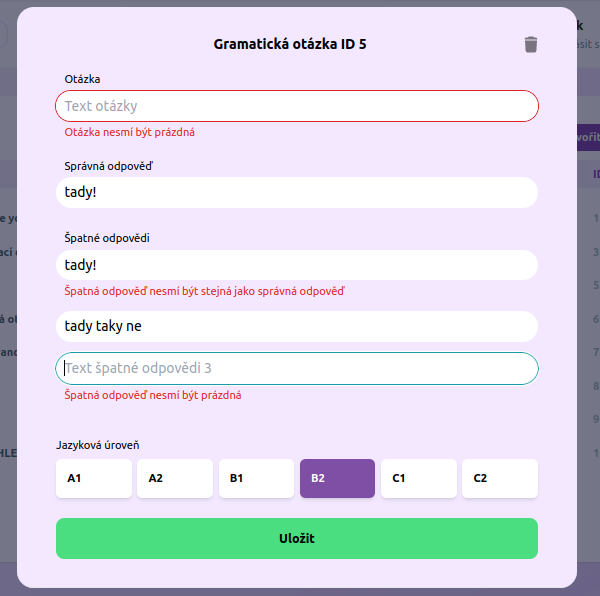
\includegraphics[width=400px]{images/01design/question-bad.png}
    \caption{Modální okno nastavení gramatické otázky s nesprávně vyplněnými hodnotami.}
\end{figure}

Pokud nejsou všechna pole vyplněna správně, nelze otázku uložit. Stále je však možné otázku smazat kliknutím na ikonku odpadkového koše v pravém horním rohu modálního okna.

\section{O programu}

Na hlavní stránce se na spodní straně obrazovky nachází odkaz na informace \M{O~programu}. Nachází se zde stručný popis toho, o čem program je, kde lze nalézt zdroj programu a kdo je aktuální správce programu (nastavitelné v konfiguraci, viz \ref{sec:config}).

\begin{figure}[H]
    \centering
    
\includegraphics[width=400px]{images/01design/about.png}
    \caption{Stránka O programu.}
\end{figure}
